\documentclass{article}

\usepackage{graphicx}
\usepackage{amsmath,amsfonts,amssymb}
\usepackage[colorlinks,bookmarks,bookmarksnumbered,allcolors=blue]{hyperref}
\usepackage[capitalise]{cleveref}
\usepackage[top=0.75in]{geometry}
\usepackage[dvipsnames]{xcolor}
\usepackage{amsmath} 
\usepackage{esvect}
\usepackage{hyperref}
\usepackage{graphicx}
\usepackage{subcaption}
\usepackage{stfloats}
\usepackage{array}
\usepackage{booktabs}
\usepackage{amsmath}

\begin{document}

\author{Joe Spencer}
\title{Rotor Optimization}
\date{November 12, 2022}
\maketitle

\subsubsection*{Methods}

This project will use an optimizer to determine which combination of design variables will be best for a propellor to meet certain requirements defined by the user. The optimizer will be confined within several limitations that will maintain it within 110\% of its original bending moment and 110\% of its original torque, to confine possible designs to the domain of real rotors that could actually be created to withstand the same loads as the original rotor.

These requirements will demonstrate that the rotor can safely fulfill its design purpose. Other requirements besides these are more flexible. These can also be modified depending on what is most important to the user. In one situation, they may be important, while in others they may not. Some of these include the power coefficient, the total power produced, the operating velocity, and the efficiency. \newline

There are several variable factors that can be adjusted and several performance measure that can still be used to determine a better propellor design. The rotor's blade length and width can be changed together or separately, depending on the situation. The blade count, shape, and twist distribution can be adjusted when the rotor is manufactured. Other variables including the rotational velocity and the angle of rotation, the angle between the tangential velocity of the rotor and the velocity of the incoming wind, can be modified during use. In this project, constraints were added to some of these values while other values were left flexible to be optimized. \newline

The values that were selected as design variables are the rotational velocity, the chord length, the twist angle, and the velocity relative to the oncoming air. Reasonable maximum limits were selected for each of these variables to keep them in the domain of reasonable solutions. Table 1 shows the maximum and minimum limits that were put in place for each of these variables to keep them in the domain of actual feasible solutions. \newline

\begin{table}[bp]
	\centering
	\title{Input Value Limits in Rotor Design \newline}
	\title{\emph{These are the maximum and minimum values that were considered in rotor design.}} \label{table:1} \newline
	\begin{tabular}{| c | c | c | c | c | c |}
		 \hline
		 \textbf{Parameter} & Minimum & Maximum \\ \hline
		 \textbf{Chord Length Magnification} & 10\% & 500\% \\ \newline
		 \textbf{Twist Angle, degrees} & $-45^{\circ}$ & $45^{\circ}$ \\ \newline
		 \textbf{Free Stream Velocity, m/s} & 0 m/s & 300 m/s \\ \newline
		 \textbf{Rotational Velocity, rpm} & 0.1 rpm & 10,000 rpm \\ \hline
	\end{tabular}
\end{table}

These requirements keep the rotor within a real range. The limits, the design variables, and other supporting values to define the rotor were put into an optimizer, which then found the optimal rotational velocity, chord length, twist angle, and air velocity for rotors with several different blade counts. The optimal rotor is found by minimizing $f(x)$ in equation 1. In this analysis, $f(x)$ represents the ratio of the rotor's thrust coefficient, $C_{T}$, its efficiency, $\eta$, and the free steam velocity, $v$, to its required power coefficient, $C_{P}$. Optimizing this function should produce a rotor that produces a lot of thrust for its required power while also being efficient and maintaining a high velocity. \newline

\begin{equation}
\begin{aligned}
	f(x_{1}, x_{2}, x_{3}...) = \frac{C_{T} \eta v}{C_{P}}
\end{aligned}
\end{equation}

The equations to find power and efficiency are already related. They both contain the power coefficient, $C_{P}$, which can be found by \hyperlink{BEM}{blade element momentum theory}. In addition, the equation for power contains the cube of the rotational velocity in revolutions per second, $n_{r}$, which is related to the rotational velocity $\omega$ in radians per second by a simple factor. \newline

\begin{equation}
\begin{aligned}
	\eta = J \frac{C_{T}}{C_{P}} \\
	P = \rho n_{r}^{3} D^{5} C_{P} \\
	\omega = n_{r} \times \frac{2 \pi}{60}
\end{aligned}
\end{equation}

In addition to the first objective function, two other objective functions were used. In these equations, thrust is represented by $T$, $\eta$ represents efficiency, $\omega$ represents rotational velocity, and $P$ is the power required by the rotor. This report will show that optimizing each function yielded a different rotor design. 

\begin{equation}
\begin{aligned}
	f(x) = \frac{T \eta \omega}{P}  \\
	f(x) = \frac{T \eta}{\omega}
\end{aligned}
\end{equation}

\subsubsection*{Results and Discussion}

\begin{table}[bp]
	\centering
	\title{Outputs of Rotor Optimization Code for Different Blade Counts \newline}
	\title{\emph{Graphs to accompany these rotors are shown in Figure 1.}} \label{table:1} \newline
	\begin{tabular}{| c | c | c | c | c | c |}
		 \hline
		 \textbf{Rotor} & Original & 2 Blades & 3 Blades & 4 Blades & 8 Blades \\ \hline
		 \multicolumn{6}{c|}{Objective Function: $ f(x) = \frac{C_{T} \eta v}{C_{P}} $} \\ \hline
		 \textbf{Chord Magnification} & 1.1 & 0.10 & 0.10 & 0.10 & 0.10 \\ \newline
		 \textbf{Twist Angle, degrees} & 1 & -0.17 & -0.16 & -0.16 & -0.14 \\ \newline
		 \textbf{Free Stream Velocity, m/s} & 20 & 300 & 300 & 300 & 300 \\ \newline
		 \textbf{Rotational Velocity, rpm} & 800 & 494.48 & 424.24 & 385.58 & 298.08 \\ \hline
		 \multicolumn{6}{c|}{Objective Function: $ f(x) = \frac{T \eta \omega}{P}  $} \\ \hline
		 \textbf{Chord Magnification} & 1.1 & 0.10 & 0.10 & 0.10 & 0.10 \\ \newline
		 \textbf{Twist Angle, degrees} & 1 & -0.16 & -0.16 & -0.16 & -0.14 \\ \newline
		 \textbf{Free Stream Velocity, m/s} & 20 & 282.79 & 25.22 & 195.08 & 152.28 \\ \newline
		 \textbf{Rotational Velocity, rpm} & 800 & 461.23 & 35.66 & 249.13 & 151.31 \\ \hline
		 \multicolumn{6}{c|}{Objective Function: $ f(x) = \frac{T \eta}{\omega} $} \\ \hline
		 \textbf{Chord Magnification} & 1.1 & 5.97 & 4.57 & 3.79 & 2.25 \\ \newline
		 \textbf{Twist Angle, degrees} & 1 & 0.27 & 0.30 & 0.31 & 0.35 \\ \newline
		 \textbf{Free Stream Velocity, m/s} & 20 & 300 & 300 & 300 & 300 \\ \newline
		 \textbf{Rotational Velocity, rpm} & 800 & 261.32 & 282.56 & 299.48 & 348.05 \\ \hline
	\end{tabular}
\end{table}

This investigation found that given certain constraints, different types of rotors are better suited to different environments. The results for each blade count are shown in table 1. This table shows that different blade counts have different optimal parameters. A visual representation of these results is found in figure 1. Several conclusions can be drawn from examining table 1 and figure 1. \newline

First off, optimal chord magnitude seemed to be constant in some cases and negatively correlated with the blade count in others. Rotors with fewer blades had an optimal chord thickness that was magnified several times.  Once optimized, even the rotor with 8 blades was nearly twice as thick as the original blade. It can be seen from this data that increasing the chord length of a blade will increase its power and efficiency at lower rotational velocities. \newline

\begin{figure}
  \centering
  \subfloat[Chord Length]{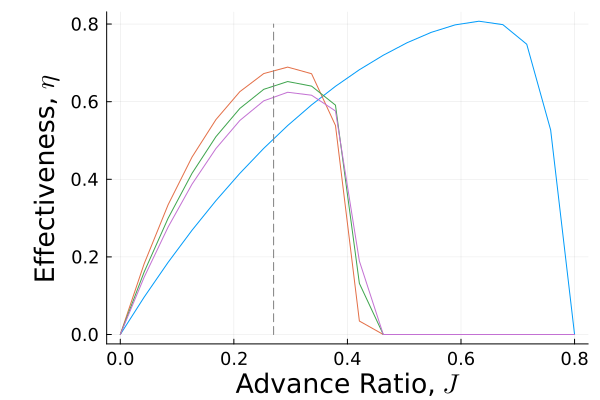
\includegraphics[width = .30\textwidth]{Plots/Figure_1.png}}
  \subfloat[Twist Angle]{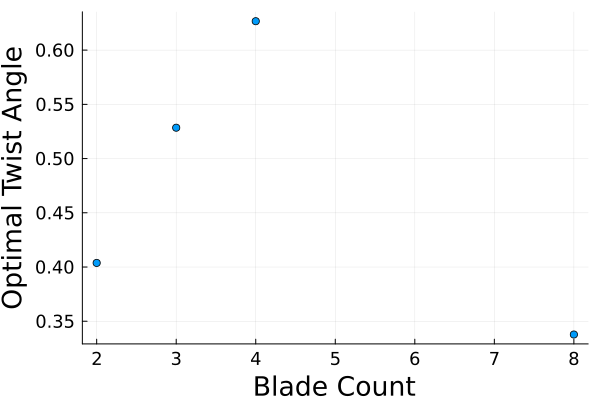
\includegraphics[width = .30\textwidth]{Plots/Figure_2.png}}

  \subfloat[Wind Velocity]{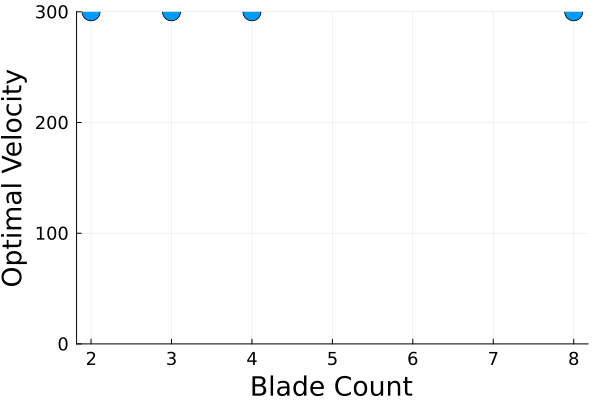
\includegraphics[width = .30\textwidth]{Plots/Figure_3.png}}\hspace{1em}
  \subfloat[Rotational Velocity]{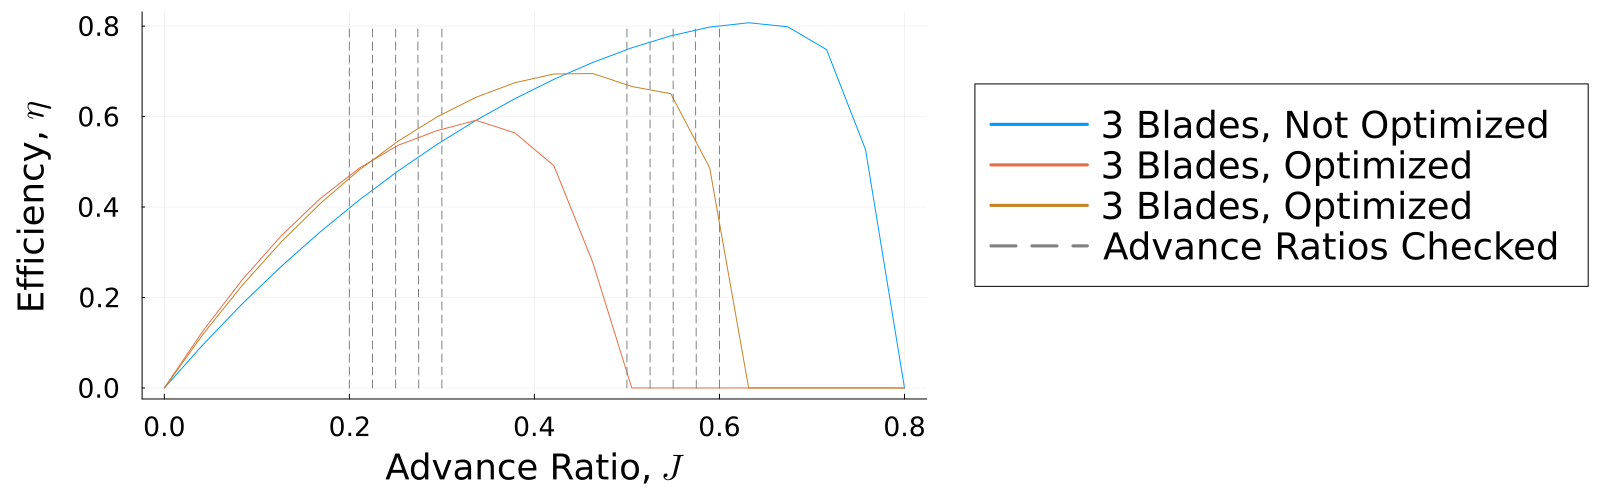
\includegraphics[width = .30\textwidth]{Plots/Figure_4.png}}
  \caption{Optimal Blade Parameters Compared With Blade Counts}
  \captionsetup{aboveskip=0pt,font=it}
  \caption*{These plots show that the optimal parameters for a turbine vary based on how many blades it has.}
  \label{fig:2}
\end{figure}

\begin{figure}
  \centering
  \subfloat[Chord Length]{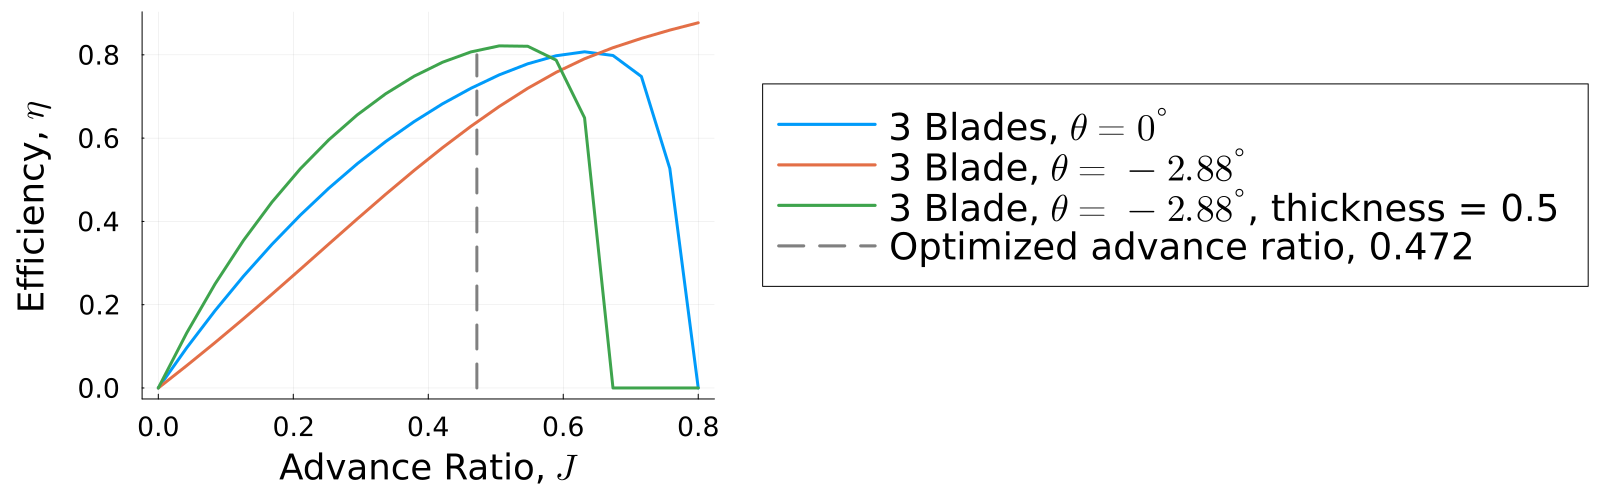
\includegraphics[width = .30\textwidth]{Plots/Figure_5.png}}
  \subfloat[Twist Angle]{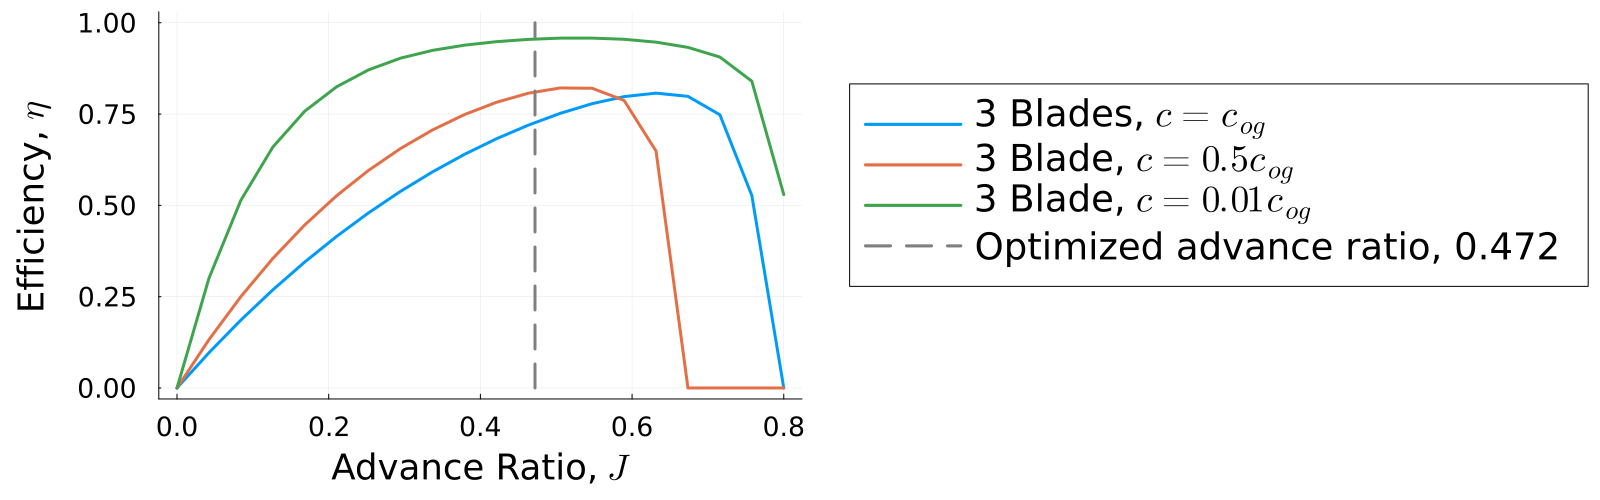
\includegraphics[width = .30\textwidth]{Plots/Figure_6.png}}

  \subfloat[Wind Velocity]{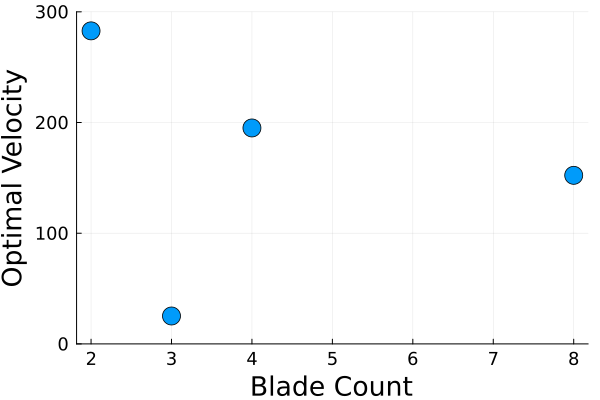
\includegraphics[width = .30\textwidth]{Plots/Figure_7.png}}\hspace{1em}
  \subfloat[Rotational Velocity]{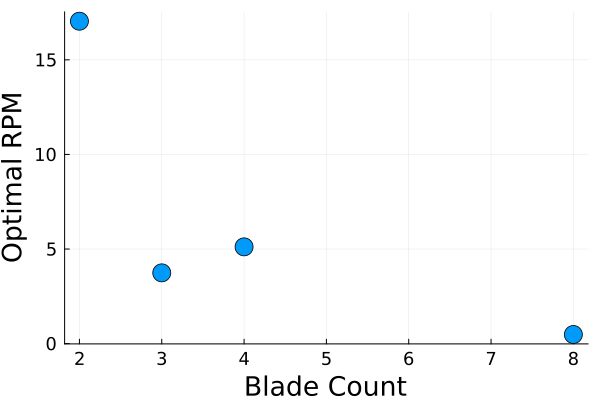
\includegraphics[width = .30\textwidth]{Plots/Figure_8.png}}
  \caption{Optimal Blade Parameters Compared With Blade Counts}
  \captionsetup{aboveskip=0pt,font=it}
  \caption*{These plots show that the optimal parameters for a turbine vary based on how many blades it has.}
  \label{fig:2}
\end{figure}

\begin{figure}
  \centering
  \subfloat[Chord Length]{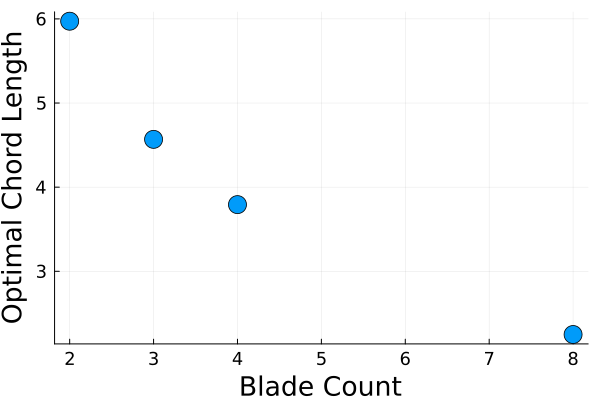
\includegraphics[width = .30\textwidth]{Plots/Figure_9.png}}
  \subfloat[Twist Angle]{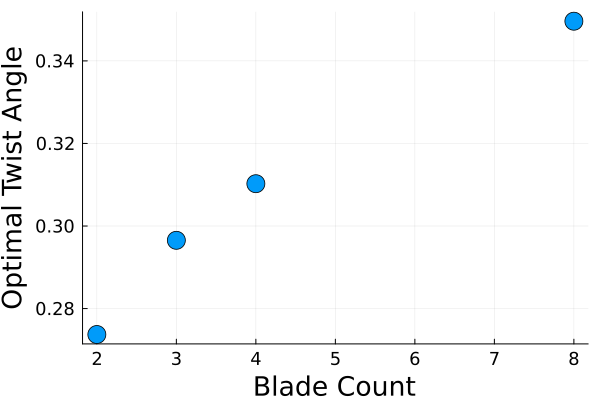
\includegraphics[width = .30\textwidth]{Plots/Figure_10.png}}

  \subfloat[Wind Velocity]{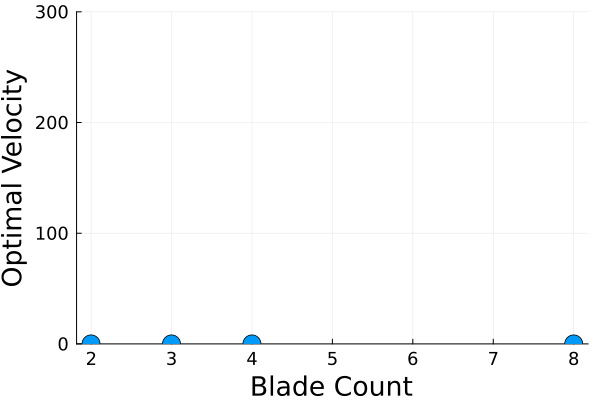
\includegraphics[width = .30\textwidth]{Plots/Figure_11.png}}\hspace{1em}
  \subfloat[Rotational Velocity]{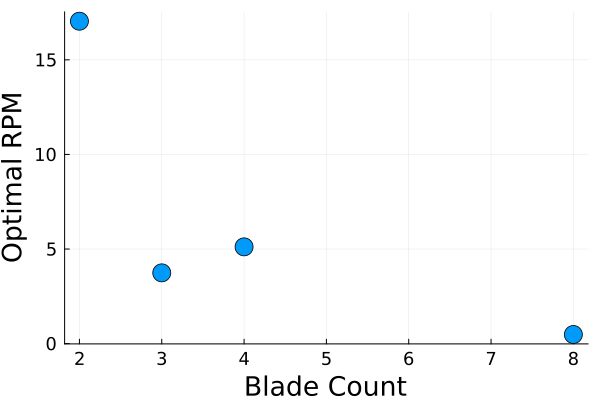
\includegraphics[width = .30\textwidth]{Plots/Figure_12.png}}
  \caption{Optimal Blade Parameters Compared With Blade Counts}
  \captionsetup{aboveskip=0pt,font=it}
  \caption*{These plots show that the optimal parameters for a turbine vary based on how many blades it has.}
  \label{fig:2}
\end{figure}

 This research had varying results when it investigated the effect of twist angle on the objective function. The optimal twist angle for each blade had a magnitude of less than one degree. In the first two functions, it was a slight negative twist, and in the third case a slight positive twist was better. The optimal rotational velocity was also consistent in the first and third cases: each rotor blade performed the objective function best at 300 m/s, which was the maximum air velocity used in this lab. In the second case, though, which found the maximum thrust compared to required power, the optimal velocity decreased as the blade count increased. \newline
 
 As the blade count of rotors increased, lower rotational velocities performed better in the first two cases and higher velocities were better in the third case. The performance relative to rotational velocity can easily be explained in the second and third cases, because it was part of the objective function itself, in the numerator and the denominator, respectively. The first case, though, found that lower rotational velocity was better for increasing the ratio of thrust and efficiency to input power. \newline
 
 This analysis optimized rotors using one equation, but other analyses could be performed for other equations using different variables, if desired. These different analyses will likely yield different results to design rotors that are better suited for unique applications. \newline

\clearpage

\section{Glossary}

This is a compilation of the previous two glossaries that I have included in my previous \href{https://github.com/JoeSpencer1/497R-Projects/blob/Rotor-Analysis/Airfoil Analysis/Airfoil_Analysis.pdf}{Airfoil Analysis} and \href{https://github.com/JoeSpencer1/497R-Projects/blob/Rotor-Analysis/Rotor Analysis/Rotor_Analysis.pdf}{Rotor Analysis} reports.

\begin{itemize}
	
	\item \hypertarget{J}{Advance Ratio, $J$} - A rotor's advance ratio is a non-dimensional term. It describes the ratio how quickly a rotor is moving relative to the fluid flowing past it. A high advance ratio signifies that either the fluid is moving quickly or the rotor is moving slowly. It is modeled by the following equation, in which $V_{a}$ is the free stream fluid velocity, $n$ is the rotational velocity, and $D$ is the rotor diameter.
	\begin{equation}
	\begin{aligned}
		J = \frac{V_{a}}{n D}
	\end{aligned}
	\end{equation}
		
	\item \hypertarget{alpha}{Angle of Attack, $\alpha$} - The angle of attack, $\alpha$ is the angle between the motion of oncoming fluid and the chord line of the airfoil. a positive $\alpha$ corresponds to a airfoil tilted upwards.
	
	\item \hypertarget{phi}{Angle of Rotation, $\phi$} - The angle of rotation, sometimes denoted by the Greek letter $\phi$, is the angle between the freest stream velocity and the velocity of the airfoil as it rotates. It is used in \hyperlink{BEM}{blade element momentum theory} calculations.

	\item \hypertarget{a}{Axial Induction Factor, $a$} - The axial induction factor is the ratio of the reduction in air velocity at an airfoil to its free stream velocity.
	
	\item \hypertarget{M}{Bending Moment, $M$} - The bending moment a rotor experiences can be modeled by integrating the shear force it is exposed to with respect to its distance in the x-direction. 
	
	\item \hypertarget{BEM}{Blade Element Momentum Theory} - The theory used to calculate local forces on a propellor or wind turbine blade. It employs both \hyperlink{BET}{blade element theory} and \hyperlink{MT}{momentum theory}. These equations are used to recursively find the \hyperlink{a}{axial induction factor, $a$}, \hyperlink{a'}{tangential induction factor}, and \hyperlink{phi}{angle of rotation, $\phi$}
	\begin{equation}
	\begin{aligned}
		\frac{1}{2} W^{2} N c C_{y} = 4 \pi U_{\infty} (1 - a) \times \Omega a' r^{2} \\
		\frac{1}{2} \rho W^{2} N c C_{x} = 4 \pi \rho [(a' \Omega r)^{2} + \Omega^{2}_{\infty} a (1 - a)] r \\
		\sin \phi = \frac{U_{\infty}}{W} (1 - a)
	\end{aligned}
	\end{equation}
In these equations, $a$, $a'$, and $\phi$ are the previously mentioned axial and tangential induction factors and angle of rotation. The airfoil's apparent speed is represented by the letter $W$, $N$ is the number of propellers, $\rho$ is the fluid density, $c$ is the chord length, $C_{x}$ and $C_{y}$ are obtained by the equation below, $U_{\infty}$ is the fluid free velocity, $\Omega$ is the blade's angular speed, and $r$ is the radius to the tip of the blade.
	\begin{equation}
	\begin{aligned}
		C_{x} = c_{l} \cos{\phi} + c_{d} \sin{\phi} \\
		C_{y} = c_{l} \sin{\phi} + c_{d} \cos{\phi}
	\end{aligned}
	\end{equation}
	
	\item \hypertarget{BET}{Blade Element Theory} - Blade element theory calculates the forces on a turbine blade by dividing it into finite pieces and summing the forces on all of these pieces. This theory determines the induced velocity and efficiency of a point along a blade using these equations:
	\begin{equation}
	\begin{aligned}
		v_{i} = \sqrt{\frac{T}{A} \frac{1}{2 \rho}} \\
        		\eta = \frac{\tan{\phi}}{\tan{(\phi + \gamma)}}
	\end{aligned}
	\end{equation}
In these equations, $v_{i}$ is the uniform induced velocity across the disk, $T$ the thrust it experiences, $A$ is its area, $\rho$ is the air density, $\phi$ is the angle to the airfoil's plane of rotation as it moves forward, and $\gamma$ is the difference between $\phi$ and $\beta$, what the airfoil's actual angle of rotation would be if it were stationary.
	
	\item \hypertarget{Camber}{Camber} - An airfoil's camber is represented by the camber line, which runs halfway between its top and bottom surfaces. This line represents the curvature of an airfoil. An airfoil with positive camber is slightly convex on top and slightly concave on its bottom.
	
	\item \hypertarget{c}{Chord, $c$} - An airfoil's chord is the imaginary line running straight from the leading edge of an airfoil to its trailing edge. The chord line is used to find an airfoil's \hyperlink{alpha}{angle of attack}. The chord length distribution shows the length of a rotor's chord at different angular positions around itself. An airfoil with a constant angle of attack $\alpha$ as it generates lift has an elliptic chord distribution.

	\item \hypertarget{CD}{Drag Coefficient (2D), $c_{D}$} - The drag coefficient determines how much drag force opposing motion will be experienced. It comes from a combination of \hyperlink{DP}{pressure drag}, also called form drag, and \hyperlink{VD}{viscous drag} or skin friction. The drag force equation describes it in this way: 
		\begin{equation} \label{eq:13}
		\begin{aligned}
        			D = \frac{1}{2} \rho u^{2} c_{D}
	    	\end{aligned}
		\end{equation}
	
	\item \hypertarget{Vinf}{Freestream Velocity, $V_{\infty}$} - The velocity of an oncoming air flow directly upstream from an airfoil, before it interacts with it.
	
	\item \hypertarget{D/D}{Hub-to-Tip Ratio} - A rotor's hub-to-tip ratio divides the distance along the blade that is actually exposed wind by the entire length of the blade. This needs to be taken into account when calculating constants like the airfoil's \hyperlink{lambda}{tip speed ratio}.
		
	\item \hypertarget{CL}{Lift Coefficient (2D), $c_{L}$} - The lift coefficient is used in the equation below to define how much lift force acts perpendicular to the direction of the oncoming fluid flow.
		\begin{equation} \label{eq:14}
		\begin{aligned}
        			L = \frac{1}{2} \rho u^{2} c_{L}
	    	\end{aligned}
		\end{equation}
	
	\item \hypertarget{LC}{Lift Curve Slope} - The lift curve plots the \hyperlink{CL}{lift coefficient} against the \hyperlink{alpha}{angle of attack} for a single airfoil. This shows the effect that changing the angle of attack will have on the airfoil's total lift force, which can be combined with other airfoils in the case of a wing to find the total lift force experienced by the wing.
		
	\item \hypertarget{M}{Mach Number, $M$} - The mach number is the velocity of an object in proportion to the speed of sound in its medium. When an airfoil is traveling near the speed of sound, its top portions can have fluid velocity above mach 1. When an airfoil is traveling above mach 1, the fluid on both sides of it also have velocities above mach 1 while there are points directly before and after it that are below mach 1.
		\begin{equation} \label{eq:15}
		\begin{aligned}
        			M = \frac{u}{c}
	    	\end{aligned}
		\end{equation}
	
	\item \hypertarget{MT}{Momentum Theory} - Momentum theory defines the power required to produce sufficient thrust to maintain momentum in a blade by the following equation, where $T$ is thrust, $\rho$ is density, $A$ is disc area, and $P$ is power:
	\begin{equation}
	\begin{aligned}
        		P = \sqrt{\frac{T^{3}}{2 \rho A}}
	\end{aligned}
	\end{equation}
		
	\item \hypertarget{NACA}{NACA Airfoil (4-Digit)} - A airfoil shape developed by the National Advisory Committee for Aeronautics (NACA). The first digit is the maximum \hyperlink{Camber}{camber} in tenths of the \hyperlink{c}{chord}. The second digit is the distance in tenths of the maximum camber from the leading edge, out of ten. the final two digits are the maximum airfoil thickness as a percentage of the chord. Descriptions of other NACA numbers can also be found on this \href{https://en.wikipedia.org/wiki/NACA_airfoil}{wikipedia article}. 
		
	\item \hypertarget{CM}{Pitching Moment Coefficient (2D), $c_{M}$} - The moment coefficient is used to calculate the pitching moment a airfoil will experience from its dynamic pressure $q$, area $S$, and chord length $c$.
		\begin{equation} \label{eq:16}
		\begin{aligned}
        			M = q S e c_{M}
	    	\end{aligned}
		\end{equation}

	\item \hypertarget{AP}{Polar} - The airfoil polar is a plot displaying the  \hyperlink{CL}{lift} and  \hyperlink{CD}{drag} coefficients corresponding with each \hyperlink{alpha}{angle of attack} for an airfoil. Examining the ratios of lift to drag is instrumental in choosing the optimal angle of attack.
	
	\item \hypertarget{PFC}{Potential-Flow Code} - A potential-flow code calculates the \hyperlink{CL}{lift}, \hyperlink{CD}{drag}, and \hyperlink{CM}{moment} forces an airfoil experiences at many different points along it. Potential-flow theory assumes constant, incompressible, inviscid fluid flow. It calculates the coefficient for each of these small points and then combines them to find the coefficients along the entire airfoil.
	
	\item \hypertarget{CP}{Power Coefficient, $C_{P}$} - A propellor's coefficient of power signifies how efficient a wind turbine is. It is the ratio of the power generated by a wind turbine to the total power of the wind flowing through it. The power generated or absorbed by an airfoil can be described by the following equation, where $P$ is power, $C_{P}$ is the coefficient of power, $\rho$ is fluid density, $n$ is the velocity in revolutions per second, and $D$ is the propellor diameter. The power coefficient and the \hyperlink{CT}{torque coefficient} are proportional to each other by a factor of $2\pi$.
	\begin{equation}
	\begin{aligned}
		P = \rho n^{3} D^{5} C_{P} \\
		C_{P} = 2 \pi C_{Q}
	\end{aligned}
	\end{equation}
		
	\item \hypertarget{DP}{Pressure Drag} - Pressure drag, also called form drag, comes from the the formation of a vacuum behind an object. The object experiences higher pressure ahead of it than behind it, so the pressure difference pushes it backwards.
	
	\item \hypertarget{APC}{Propellor Identification} - A propellor is identified by 2 numbers, which represent its diameter and its pitch, both in inches. For example, an APC 10x7 propellor is made by Advanced Precision Composites. It has a 10-inch diameter and a 7-inch pitch per revolution.
	
	\item \hypertarget{Re}{Reynolds Number, $Re$} - The Reynolds number is a unit-less number for fluid flow described by the equation below. It can be used to predict patterns in the fluid's flow, using its flow speed $u$, characteristic length $L$, and kinetic viscosity $\nu$, or else by its density $\rho$, flow speed $u$, characteristic length $L$, and fluid density $\mu$.
		\begin{equation} \label{eq:17}
		\begin{aligned}
        			Re = \frac{uL}{\nu} \\
			= \frac{\rho uL}{\mu} 
	    	\end{aligned}
		\end{equation}
	
	\item \hypertarget{sigma}{Rotor Solidity, $\sigma$} - Rotor solidity describes the ratio of a turbine's chord length, $c$, to its spacing, $s$. This is found by the following equation, in which $n_{b}$ is the number of blades, $r_{h}$ is the hub radius, and $r_{t}$ is the tip radius.
	\begin{equation}
	\begin{aligned}
		\sigma = \frac{c}{s} = \frac{c n_{b}}{2 \pi \sqrt{\frac{r^{2}_{h} + r^{2}_{t}}{2}}}
	\end{aligned}
	\end{equation}
	
	\item \hypertarget{ST}{Stall} - Stall occurs when an airfoil's \hyperlink{alpha}{angle of attack} is too great in magnitude, either positive or negative. When the angle of attack is too dramatic, flow separation occurs, reducing rather than augmenting the airfoil's \hyperlink{CL}{lift coefficient} as the angle of attack increases.
	
	\item \hypertarget{a'}{Tangential Induction Factor, $a'$} - The tangential induction factor is the ratio of the increase in air velocity tangential to the airfoil to its free stream velocity.
	
	\item \hypertarget{Th}{Thickness} - An airfoil's thickness can be measured in two different ways, either along its \hyperlink{c}{chord line} or along its \hyperlink{Camber}{camber line}. Thickness measured perpendicular to the camber line is also called the American convention, and thickness measured perpendicular to the chord line is also called the British convention.
	
	\item \hypertarget{CT}{Thrust Coefficient, $C_{T}$} - A rotor's thrust coefficient determines how much thrust in the forward direction an airfoil experiences. Thrust force is directly opposite drag. Please note the similarities and differences between the thrust equation and the \hyperlink{CP}{power equation}.
	\begin{equation}
	\begin{aligned}
		T = \rho n^{2} D^{4} C_{T}
	\end{aligned}
	\end{equation}
	
	\item \hypertarget{lambda}{Tip Speed Ratio, $\lambda$} - A wind turbine's tip speed ratio is the inverse of its \hyperlink{J}{advance ratio, $J$}. It represents the ratio of the speed of the tip of a turbine blade, or $\omega R$, to the wind speed, $v$.
	\begin{equation}
	\begin{aligned}
		\lambda = \frac{\omega R}{v} = \frac{\pi}{J}
	\end{aligned}
	\end{equation}
	
	\item \hypertarget{CQ}{Torque Coefficient, $C_{Q}$} - A rotor's torque coefficient defines how much torque it will experience. A propellor's torque is given by the following equation, in which $Q$ represents torque, $\rho$ is the fluid density, $n$ is the velocity in revolutions per second, $D$ is the diameter, and $C_{Q}$ is the coefficient of torque. The torque coefficient and the \hyperlink{CP}{power coefficient} are proportional to each other by a factor of $2\pi$.
	\begin{equation}
	\begin{aligned}
		Q = \rho n^{2} D^{5} C_{Q} \\
		C_{Q} = \frac{C_{P}}{2 \pi}
	\end{aligned}
	\end{equation}
	
	\item \hypertarget{eta}{Efficiency, $\eta$} - The efficiency of a rotor can be described by the following equation, in which $J$ is the rotor's \hyperlink{J}{advance ratio}, $C_{T}$ is its \hyperlink{CT}{thrust coefficient}, and $C_{P}$ its \hyperlink{CP}{power coefficient}:
	\begin{equation}
	\begin{aligned}
		\eta = J \frac{C_{T}}{C_{P}}
	\end{aligned}
	\end{equation}
	
	\item \hypertarget{T}{Twist Distribution} - Twist distribution along a wing redirects where air flows past it. This causes changes in both the magnitude and location lift and drag forces it experienced as air flows past it.
	
	\item \hypertarget{VD}{Viscous Drag} - Viscous drag, also called skin friction, is drag caused by friction with the fluid particles flowing past an airfoil. Along with \hyperlink{PD}{pressure drag}, it contributes to an airfoil's total \hyperlink{CD}{drag coefficient} airfoil.
	
\end{itemize}

\end{document}